\textbf{Data and manual data handling} \newline
Data used in this study were collected beforehand from an on-going FOXH trial which is conducted in collaboration with Danish and Australian universities. The data consists of pain maps which were drawn by individuals with PFPS through the use of an application, Navigate Pain, in a clinical setting. The pain maps are both from individuals with uni- and bilateral PFP, an example of these are shown in figure \ref{fig:twoPainmaps}.

\begin{figure}[h]
\centering
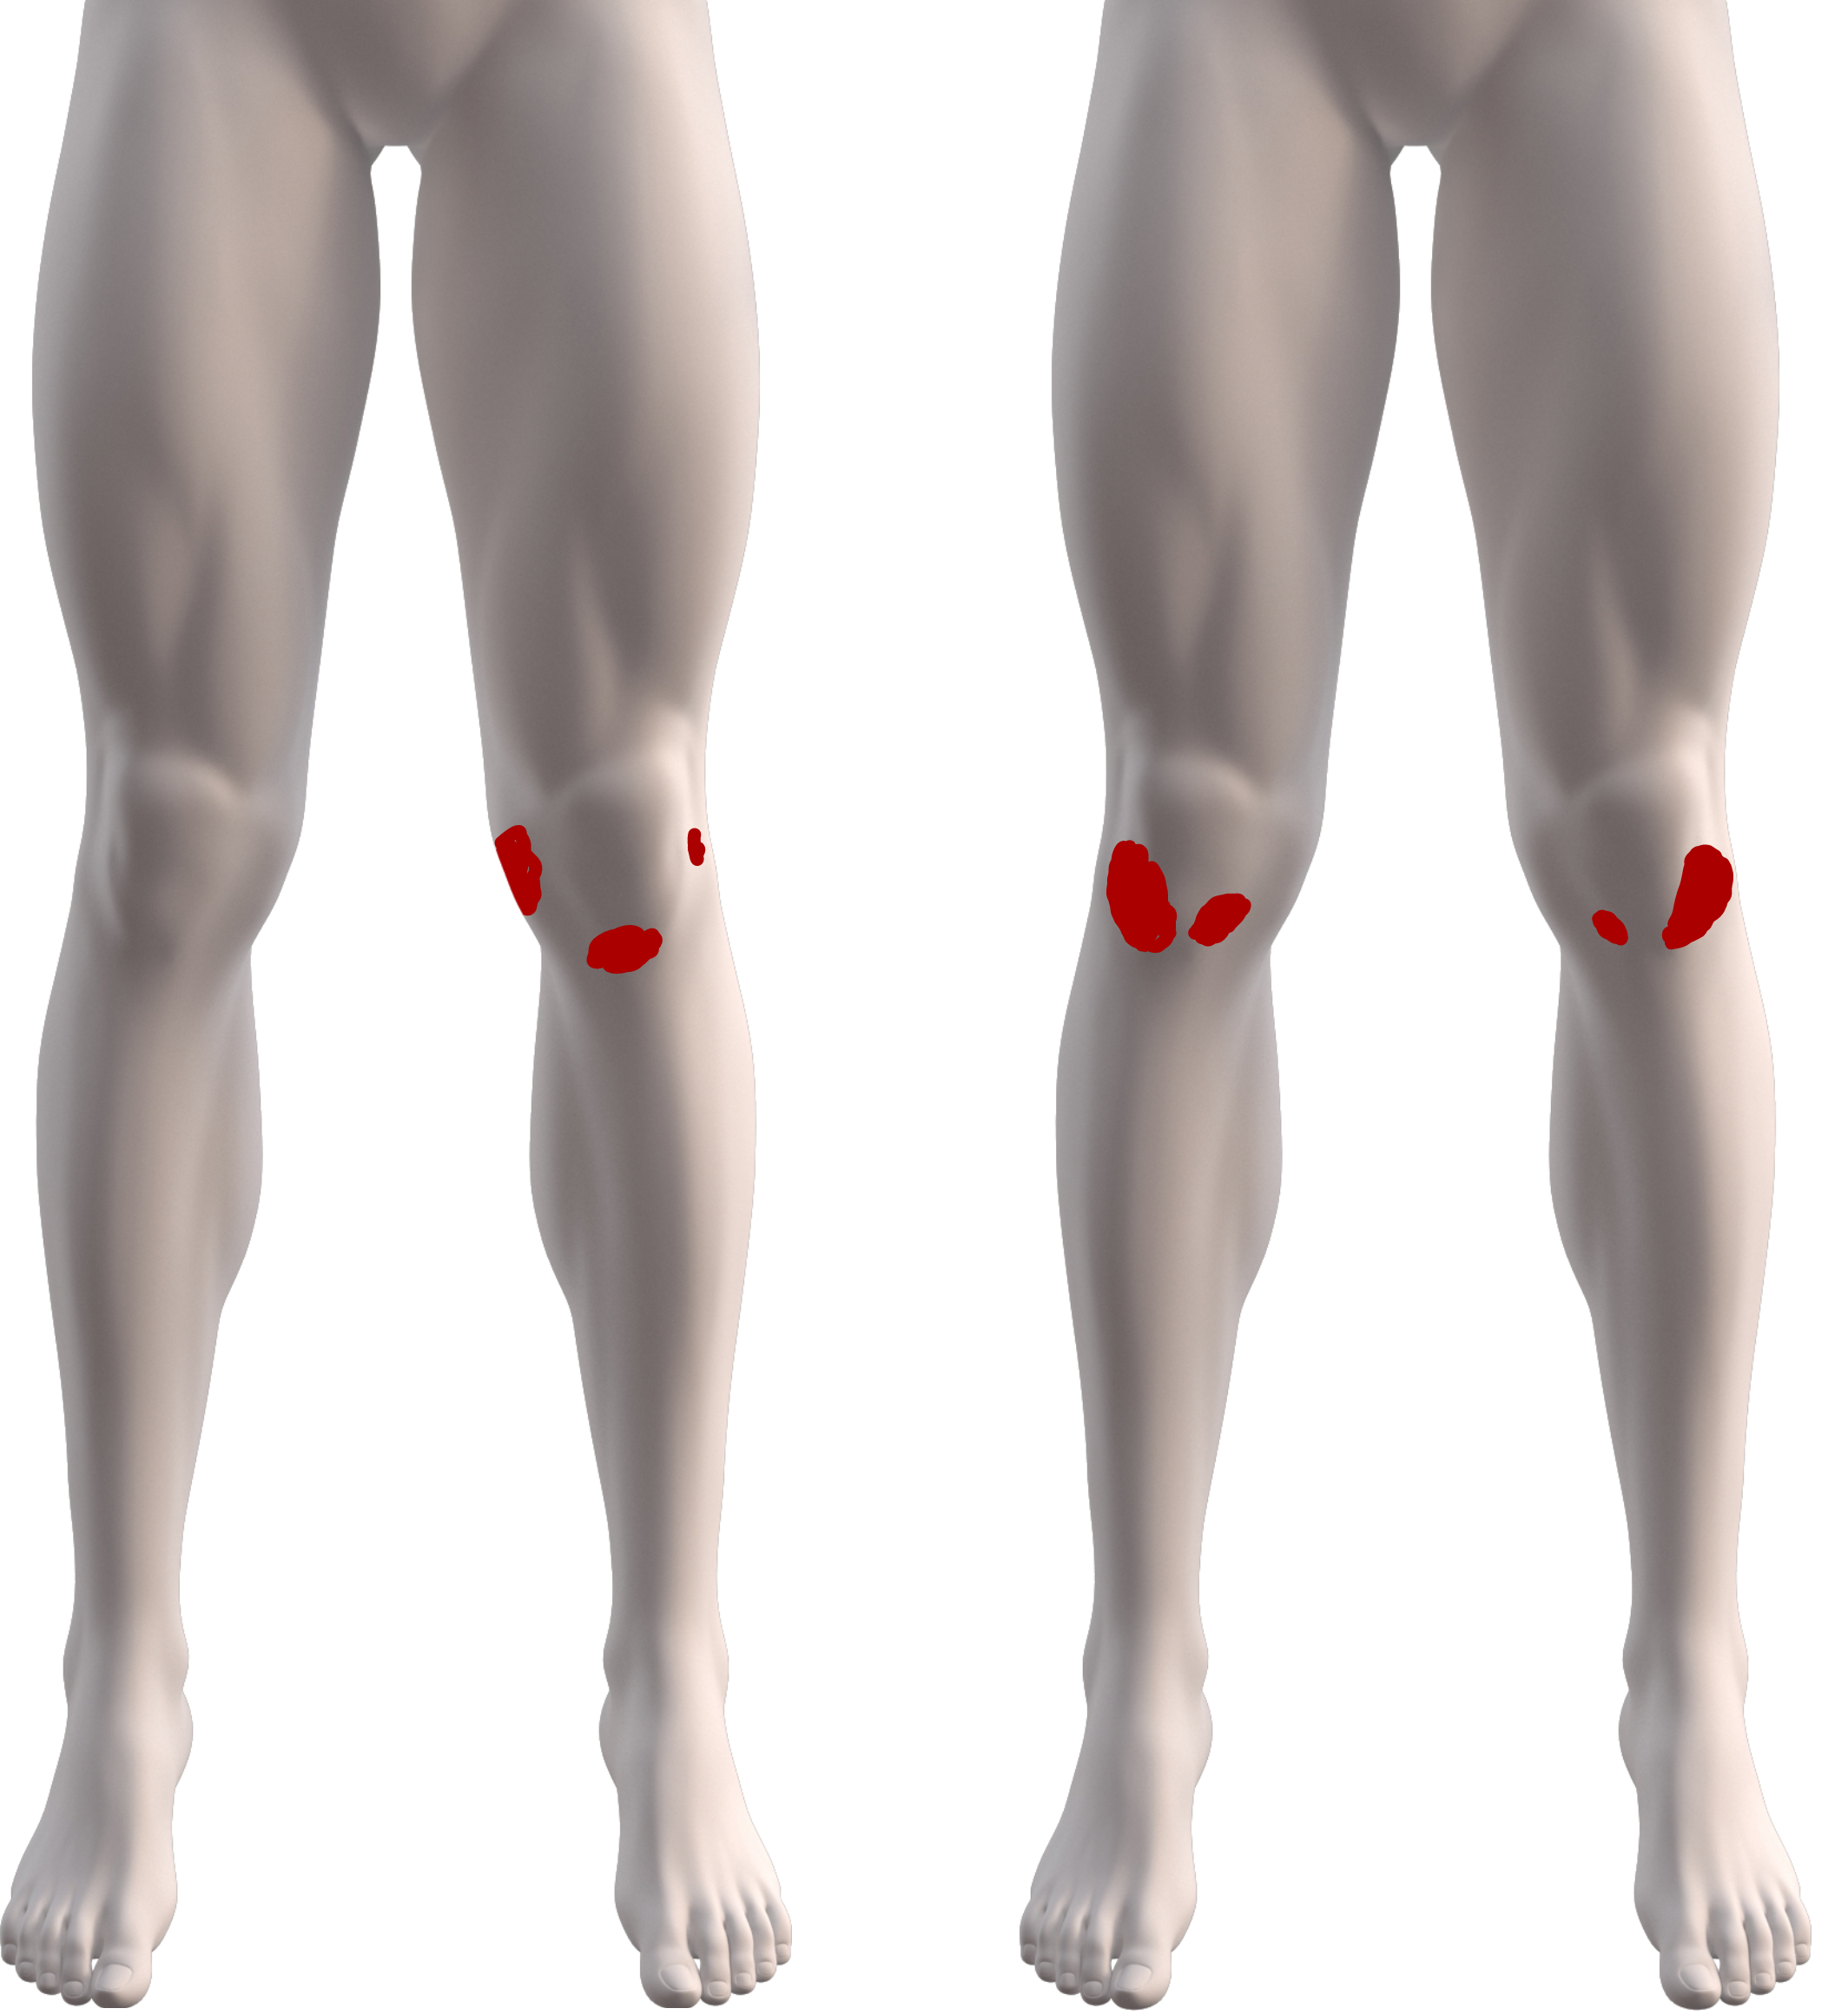
\includegraphics[width=0.4\textwidth]{Figures/twoPainmaps}
\caption{Pain maps of the lower extremities from individuals with uni- and bilateral PFP. The red markings indicate the area of pain perceived by the individuals.}
\label{fig:twoPainmaps}
\end{figure}

\noindent
In addition to the pain maps appurtenant information was available, which contained information regarding the individuals.
Before using the data in the deep learning models, a manual data handling was necessary. This incorporated matching the given pain maps and appertaining ID regarding the individuals, which resulted in 217 available pain maps. Furthermore, specific information like gender, symptom duration and pain intensity were collected from the appurtenant information. The number of pain maps with associated information, gender and symptom duration, was 205. Additionally, there were 197 pain maps with associated information, gender and pain intensity.\\

\noindent
\textbf{Software application: Navigate Pain} \newline
Navigate Pain is a software application that is used to visualise the location, shape and spatial distribution of pain from individuals to healthcare personnel. The application permits individuals to draw their pain into a body outline with different colors and line thickness. Navigate Pain android was developed at Aalborg University and a commercial web application is available at Aglance Solutions (Denmark).\citep{Solutions2015}\\

\noindent
\textbf{Data representations} \newline
It is presumed that different representations of the pain maps affect the performance accuracy of a deep learning models, which is why different data representations are created.
A study by \citeauthor{Boudreau2017} found a correlation between a prolonged symptom duration and the size of the pain area. It was shown that the pain area increased for individuals that have a symptom duration for longer than five years compared to those with a symptom duration below. Likewise, pain intensity had a correlation with the size of pain area for individuals. Furthermore, the morphology of the pain developed from a U-shape to an O-shape for individuals with a symptom duration above five years.\citep{Boudreau2017} \\
Based on this study the morphology of PFP is considered to be relevant to investigate, and therefore the morphology constitutes a data representation.

\noindent
The PFP is often described as diffuse pain and therefore difficult to describe and localise \citep{Witvrouw2014}. To accommodate this is it chosen to divide the pain into different knee regions, which may indicate whether a specific region of the knee influence the PFP. This is converted to a simplified data representation that indicate active pain regions.
A combination of the morphology and location of the pain constitutes third data representation.
\noindent
Furthermore, gender is an interesting parameter to use as an input, because the prevalence is more than twice as high for females than males. Thereto, perceived pain is subjective and depends on the individual's character and personality. The distribution of gender is investigated by creating a histogram, which showed that the prevalence is higher for females than males, given that females constitute 156 of the 206 individuals.

\noindent
It is chosen to classify the three data representation in proportion to symptom duration, based on the study by \citeauthor{Boudreau2017} which indicated that symptom duration seems to affect the size and morphology of the pain area. Furthermore the study showed that there was a correlation between pain intensity and size of pain area, which is why it is chosen to classify pain maps according to pain intensity. The three data representations are referred to as morphology-, regions- and combined-representation.\\

\noindent
\textbf{Knee regions} \newline
\noindent
Patients with PFPS often describe the knee pain as a diffuse pain, and when looking at pain drawing samples from multiple patients it is also evident that there is a high variability in the distribution of pain patterns across different areas of the knee. To distinguish between different pain areas, the knee can be divided into various regions as seen in figure \ref{fig:atlas}, where the division of the left and right anterior knees are illustrated. 

\begin{figure} [h] 
\centering
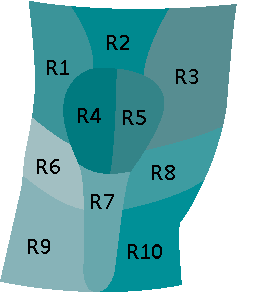
\includegraphics[width=0.5\textwidth]{Figures/atlas}
\caption{The regions of the left and right knees, where each knee is split into ten regions.}
\label{fig:atlas}
\end{figure}

\noindent
The divisions is inspired by Photographic Knee Pain Map (PKPM) which is designed to categories location of knee pain, diagnostic and research purposes. PKPM represent both knees that makes it possible to identify unilateral and bilateral pain.\citep{Elson2010}

\noindent
The regions are based on the anatomic structures according to the areas where individuals often indicate pain.
There is ten regions, where region 1 and 3 represent the superior lateral and superior medial areas for patella. Region 2 refers to quadriceps tendon. The patella is divided into lateral and medial regions, which are region 4 and 5. Region 6 and 8 are lateral and medial joint line areas. Patella tendor is region 7 and the two last regions, 9 and 10, are tibia lateral and medial.\citep{Elson2010}\\

\noindent
In relation to the regions-representation, it is necessary to find a threshold that decides when a knee region contains enough pain pixels to be considered active. A threshold is required to increase the confidence of an active pain region by avoiding minimal contributions e.g. small pain areas in the associated regions. Simultaneously the threshold may not be too large so that potential pain regions will not be incorporated. The threshold to indicate active pain regions is decided based on an analysis, where threshold values of 0, 5, 10 and 15 percent are tested. The analysis of the threshold is tested on five random pain maps to get a general impression of the data. Based on analysis of the five pain maps is 5 percent chosen as the threshold, that defines when a pain region is active. \\

\noindent
\textbf{Pre-processing of data}\newline
\noindent
The data is pre-processed in MatLab to prepare it to the three different deep learning models. Each model has an appurtenant data representation which are prepared in three different ways. In general are the pain maps resized, since it was collected at different resolutions (screen sizes) and cropped to sort out unnecessary data like the areas inferior and superior to the knee. Each data representation is reflected in a matrix consisting of the pain maps, gender and the output, symptom duration and pain intensity. The morphology-representation is not further processed before using it in the models. 
The regions-representation is a simplified representation of morphology of the pain and reflects only the active pain regions. Thereto is a threshold used to define when a region is active. The third data representation is a combination of morphology- and regions-representations, which means that the matrix reflects the morphology of the pain in each region. 

